\documentclass{beamer}
\usepackage{graphicx}
\usepackage{graphics}
\usepackage{hyperref}
\usepackage[english]{babel}
\usepackage[T1]{fontenc}
\usepackage[utf8]{inputenc}
\usepackage{xfrac}


\mode<presentation>
{
    \usetheme{AMUFree-kk}
    \setbeamercovered{transparent = 28}
}
\title{Sparse Transformers}
\date{2020}
\author{Karol Kaczmarek}
\setbeamertemplate{bibliography item}{[\theenumiv]}


\begin{document}

\begin{frame}
    \titlepage
\end{frame}

\iffalse
\AtBeginSection[]
{
    \begin{frame}
        \frametitle{Outline}
        \tableofcontents[currentsection]
    \end{frame}
}
\fi



% Transformer
\section{Transformer}
\begin{frame}
    \frametitle{Transformer \cite{transformer}}
    \begin{itemize}
        \item Transformers are powerful sequence models, but require time and memory that grows quadratically with the sequence length.
    \end{itemize}
    \begin{center}
        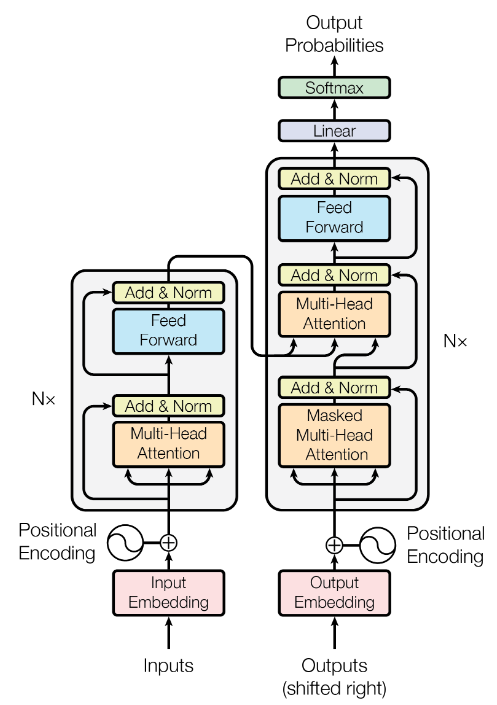
\includegraphics[scale=0.75]{img/transformer.png}
        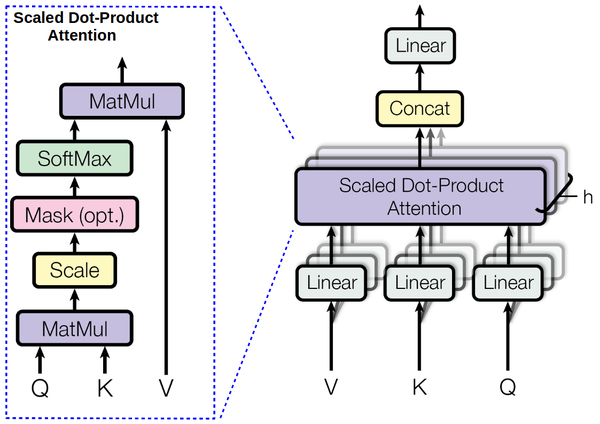
\includegraphics[scale=0.4]{img/multi_head_attention.png}
    \end{center}
\end{frame}



% Sparse Transformer
\section{Sparse Transformer}
\begin{frame}
    \frametitle{Sparse Transformer \cite{sparse_transformer}}
    \begin{itemize}
        \item April 2019, OpenAI -- code available
        \item generative model (decoder)
        \item sparse factorizations of the attention matrix (reduce to $O(n  \sqrt[p]{n})$)
        \item gradient checkpointing
        \item mixed-precision training
        \item treat images, text, and audio as a sequence of discrete tokens, typically raw bytes
    \end{itemize}
\end{frame}

\begin{frame}
    \frametitle{Factorized attention}
    \begin{center}
        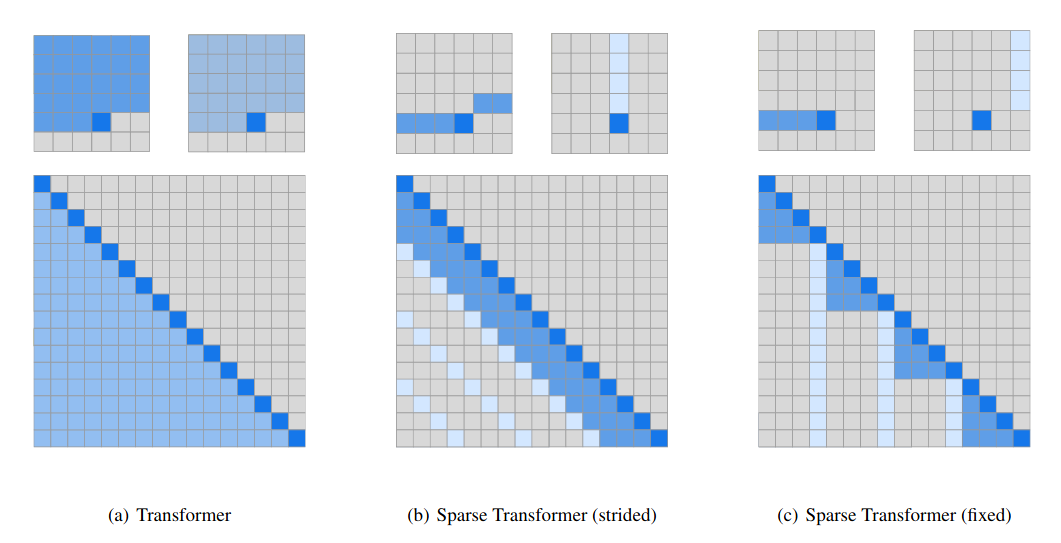
\includegraphics[scale=0.30]{img/sparse_transformer_attentions.png}
    \end{center}
\end{frame}

\begin{frame}
    \frametitle{Generating images}
    \begin{center}
        
\includegraphics[scale=0.45]{img/sparse_transformer_gen1.png}
        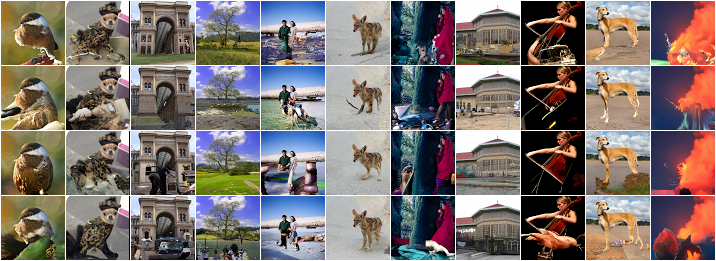
\includegraphics[scale=0.45]{img/sparse_transformer_gen2_half.png}
        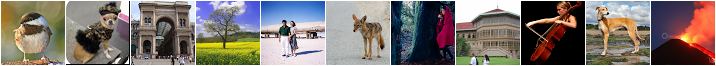
\includegraphics[scale=0.45]{img/sparse_transformer_gen3.png}
    \end{center}
\end{frame}

\begin{frame}
    \frametitle{Image GPT (iGPT) \cite{igpt} - June 2020}
    \begin{center}
        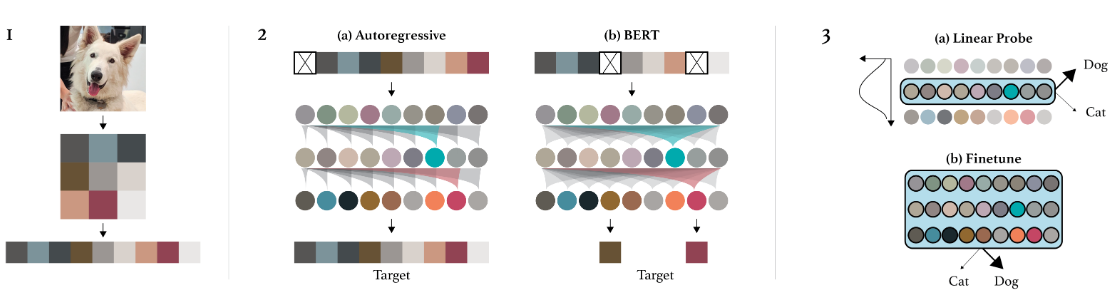
\includegraphics[scale=0.29]{img/igpt_model.png}
    \end{center}
\end{frame}

\begin{frame}
    \frametitle{Samples}
    \begin{center}
        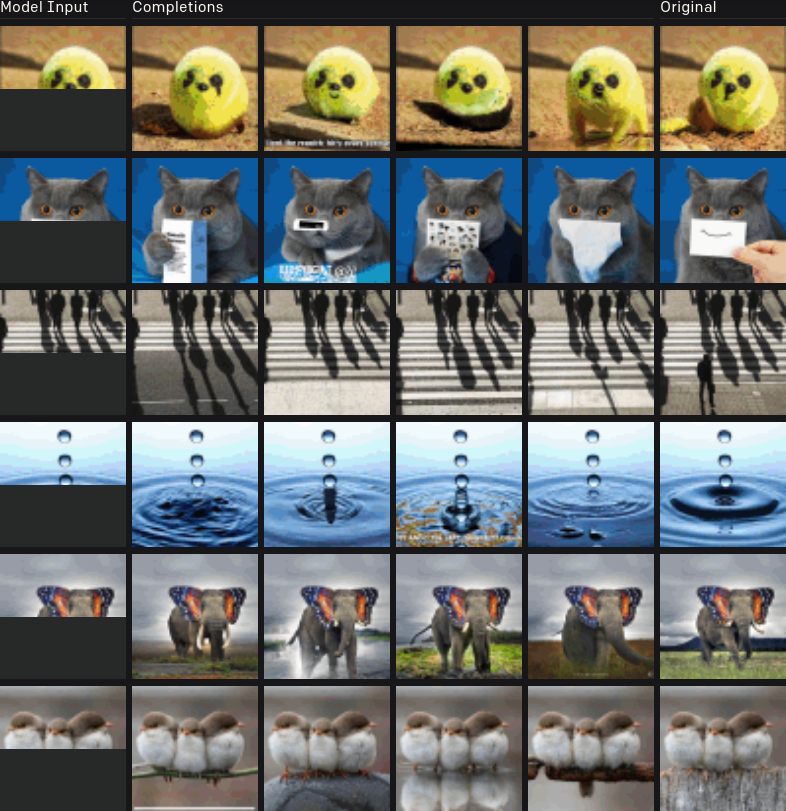
\includegraphics[scale=0.23]{img/igpt_samples.png}
    \end{center}
\end{frame}





% Synthesizer
\section{Synthesizer}
\begin{frame}
    \frametitle{Synthesizer \cite{synthesizer}}
    \begin{itemize}
        \item May 2020, Google -- source code is not available
        \item Synthetic Attention - removes the notion of query-key-values in the self-attention module and directly synthesizes the alignment matrix instead (without dot product attention or content-based attention):
        \begin{itemize}
            \item Dense Synthesizers - learns synthetic attention by conditioning on each input of $X$ and projecting to $l$ dimensions (can be interpreted as learning a token-wise projection to the sequence length $l$)
            \item Random Synthesizers - the attention weights are initialized to random values (the attention weights are not conditioned on any input tokens), learns a task-specific alignment that works well globally across many sample
        \end{itemize}
        \item use factorized version of synthetic attention
    \end{itemize}
\end{frame}


\begin{frame}
    \frametitle{Self-attention pattern}
    \begin{center}
        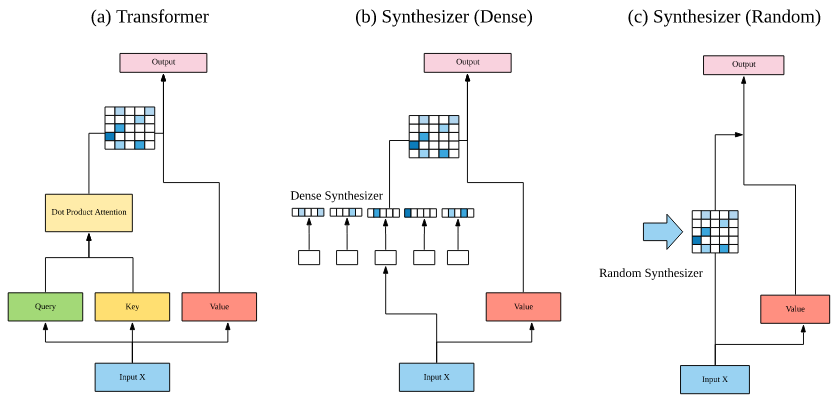
\includegraphics[scale=0.38]{img/synthesizer_attention.png}
    \end{center}
\end{frame}

\begin{frame}
    \frametitle{Synthesizer - Factorized Models}
    \begin{itemize}
        \item omit the $Q$ and $K$ projections
        \item Factorized Dense Synthesizer - split into smaller parts of input
        \item Factorized Random Synthesizer - use low rank matrices
    \end{itemize}
    \begin{center}
        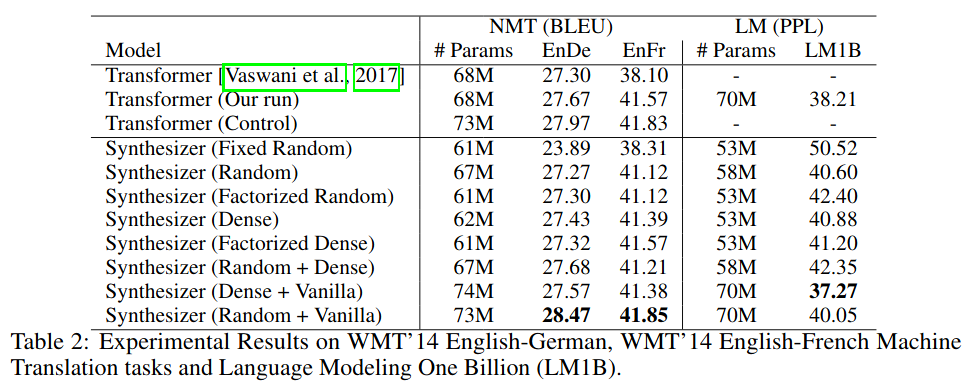
\includegraphics[scale=0.33]{img/synthesizer_score_params.png}
    \end{center}
\end{frame}

\begin{frame}
    \frametitle{T5 methodology - Score}
    \begin{center}
        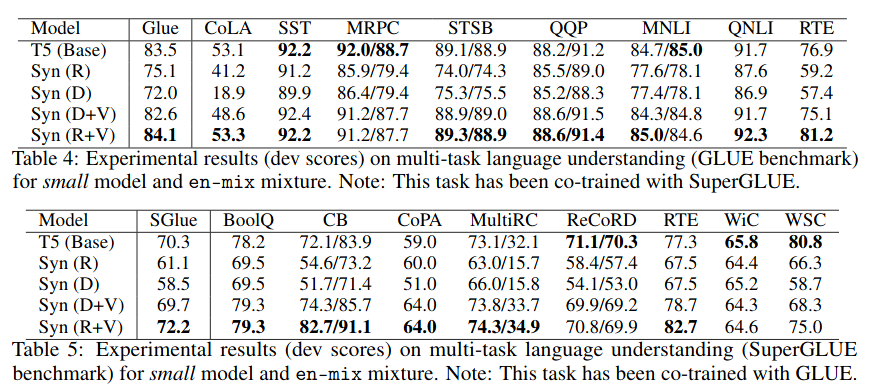
\includegraphics[scale=0.37]{img/synthesizer_score.png}
    \end{center}
\end{frame}




% Longformer
\section{Longformer}
\begin{frame}
    \frametitle{Longformer \cite{longformer}}
    \begin{itemize}
        \item April 2020, Allen Institute for Artificial Intelligence (allenai) -- available in transformers library
        \item windowed local-context self-attention (attention mechanism that scales linearly with sequence length)
        \item process long sequences without truncating or chunking
        \item autoregressive character-level language modeling (allowing the model to process sequences of up to 32K characters on modern GPUs)
        \item replace the full self-attention operation of existing pretrained models (RoBERTa model - MLM objective)
        \item custom CUDA kernel using TVM (Tensor Virtual Machine)
    \end{itemize}
\end{frame}

\begin{frame}
    \frametitle{Memory usage}
    \begin{center}
        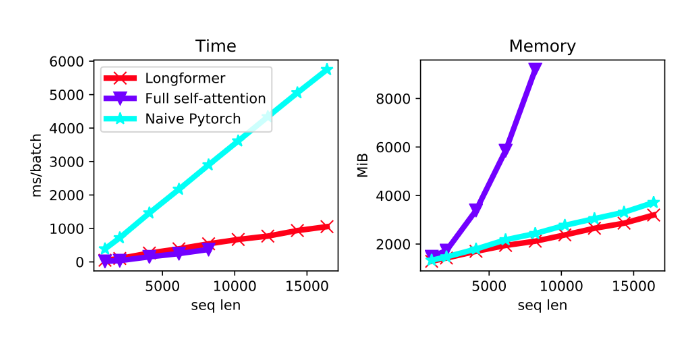
\includegraphics[scale=0.45]{img/longformer_seq_len_memory.png}
    \end{center}
\end{frame}

\begin{frame}
    \frametitle{Self-attention pattern}
    \begin{center}
        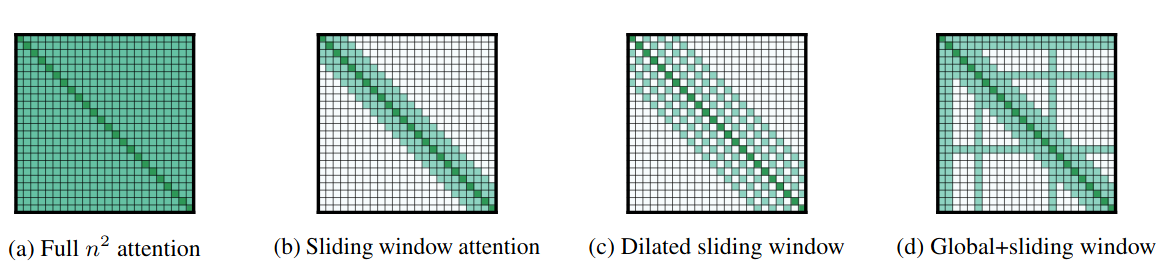
\includegraphics[scale=0.28]{img/longformer_attention.png}
    \end{center}
    \begin{itemize}
        \item Sliding Window - fixed-size window attention surrounding each token, top layers have access to all input locations
        \item Dilated Sliding Window - window has gaps of size dilation
        \item Global Attention - few pre-selected input locations (classification = [CLS] token, QA = all question tokens)
    \end{itemize}
\end{frame}

\begin{frame}
    \frametitle{AR LM - Score}
    \begin{center}
        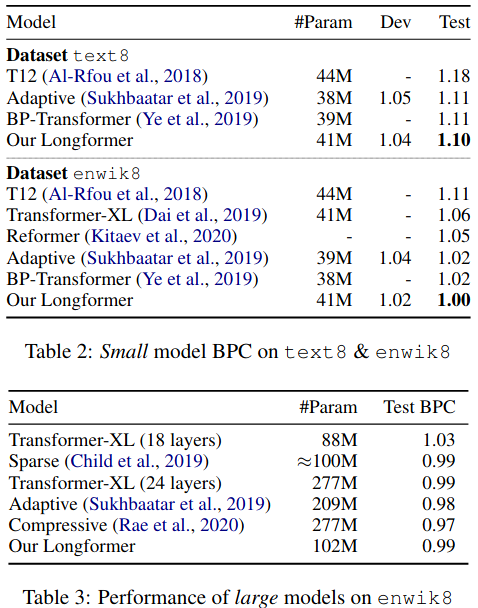
\includegraphics[scale=0.30]{img/longformer_transformer_score.png}
    \end{center}
\end{frame}

\begin{frame}
    \frametitle{RoBERTa base - Score}
    \begin{itemize}
        \item continue pre-training from the RoBERTa - use the sliding window attention with window size of 512 on all layers (uses the same amount of computation as RoBERTa)
        \item can process sequences up to 4,096 tokens long (8 times longer than BERT - 512 tokens)
        \item initialize them by copying the 512 position embedding
    \end{itemize}
    \begin{center}
        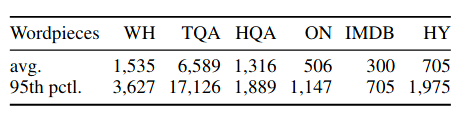
\includegraphics[scale=0.4]{img/longformer_roberta_seq_size.png}
        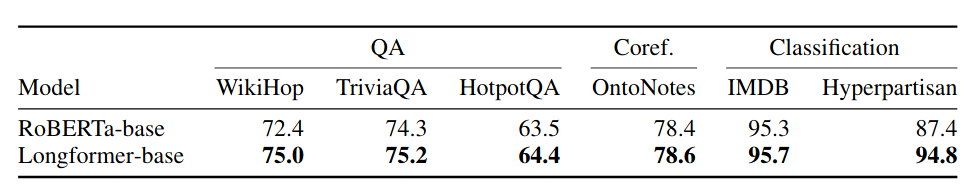
\includegraphics[scale=0.3]{img/longformer_roberta_score.png}
    \end{center}
\end{frame}




% Linformer
\section{Linformer}
\begin{frame}
    \frametitle{Linformer \cite{linformer}}
    \begin{itemize}
        \item June 2020, Facebook -- code available
        \item base on RoBERTa model
        \item self-attention mechanism can be approximated by a low-rank matrix (with different dimension for different layers - smaller dimension for higher layers)
        \item parameter sharing between projections
    \end{itemize}
    \begin{center}
        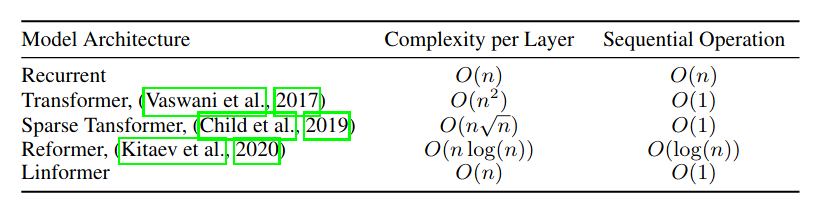
\includegraphics[scale=0.4]{img/linformer_complexity.png}
    \end{center}
\end{frame}

\begin{frame}
    \frametitle{Linformer}
    \begin{center}
        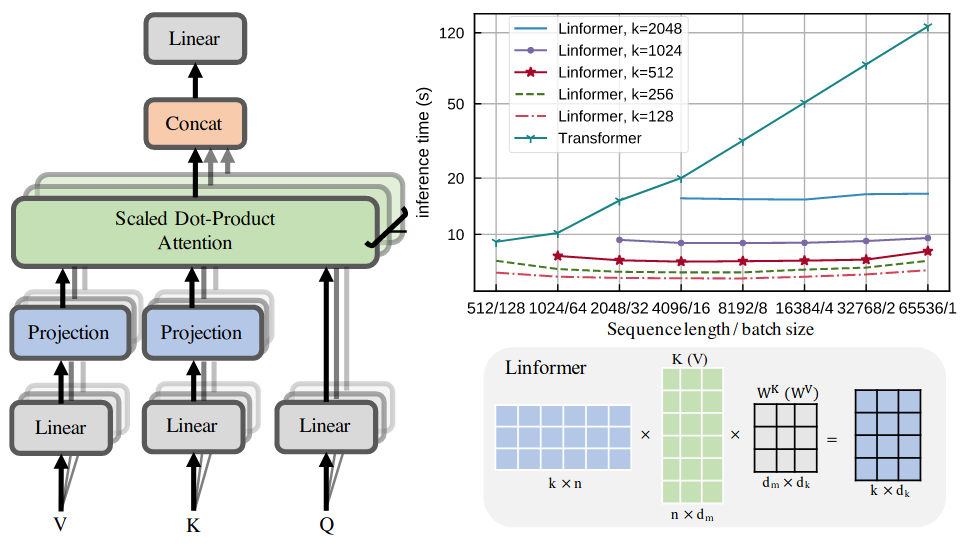
\includegraphics[scale=0.28]{img/linformer.png}
    \end{center}
    \footnotesize{if we can choose a very small projected dimension $k$, such that $k \ll n$, then we can significantly reduce the memory and space consumption}
\end{frame}

\begin{frame}
    \frametitle{Score}
    \begin{center}
        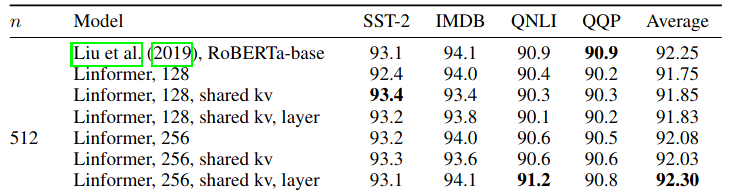
\includegraphics[scale=0.42]{img/linformer_seq_len_512_score.png}
        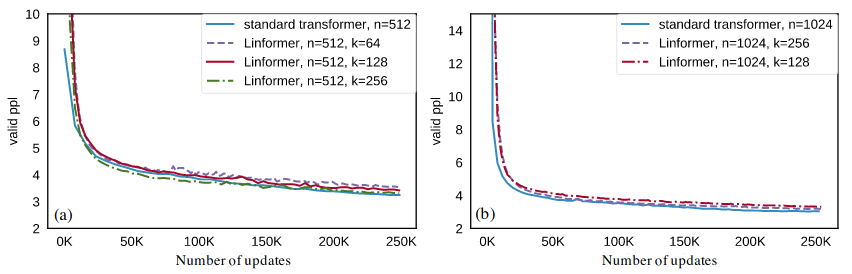
\includegraphics[scale=0.35]{img/linformer_seq_len_512_perplexity.png}
    \end{center}
\end{frame}

\begin{frame}
    \frametitle{Inference-time Efficiency Results}
    \begin{center}
        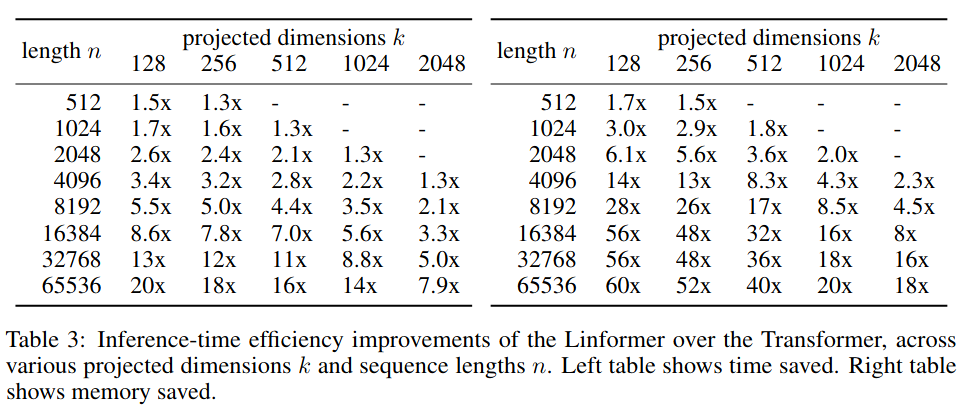
\includegraphics[scale=0.33]{img/linformer_compare.png}
    \end{center}
\end{frame}



% Others
\section{Other}
\begin{frame}
    \frametitle{Other}
    \begin{itemize}
        \item Adaptive Attention Span \cite{adaptive_span} - August 2019, Facebook
        \item Adaptively Sparse Transformers \cite{adaptively_sparse_transformers} - June 2020, Facebook
        \item Reformer \cite{reformer} - January 2020, Google
        \item nBRC \cite{n_brc} - June 2020
        \item GShard \cite{gshard}- June 30, 2020, Google
    \end{itemize}
\end{frame}


% Sandwich Transformers
\section{Sandwich Transformer}
\begin{frame}
    \frametitle{Sandwich Transformers \cite{sandwich_transformers}}
    \begin{itemize}
        \item April 2020
        \item reordering of the transformer sublayers (the sandwich reordering pattern does not guarantee performance gains across every task)
        \item test on WikiText-103
    \end{itemize}
    Each transformer layer (encoder) consists of a self-attention sublayer (s) followed by a feedforward sublayer (f):
    \begin{center}
        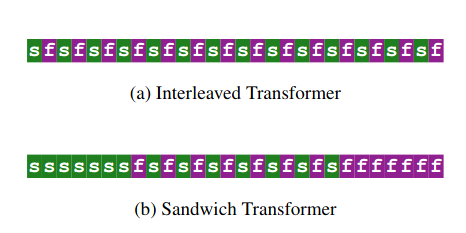
\includegraphics[scale=0.38]{img/sandwich_transformers.png}
    \end{center}
\end{frame}

\begin{frame}
    WikiText-103 -- Randomly generated models with 16 self-attention (s) sublayers and 16 feedforward (f) sub-layers
    \begin{center}
        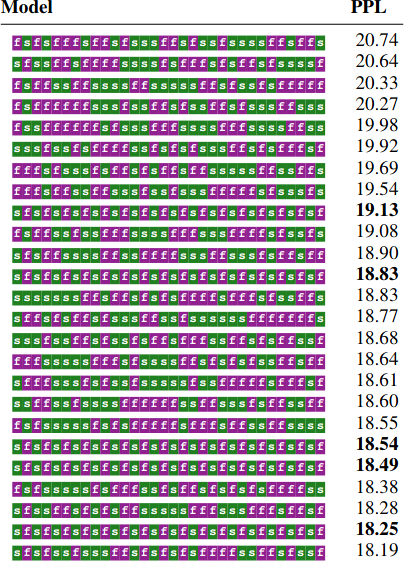
\includegraphics[scale=0.34]{img/sandwich_transformers_models1.png}
    \end{center}
\end{frame}

\begin{frame}
    WikiText-103 -- Randomly generated models with the same number of parameters
    \begin{center}
        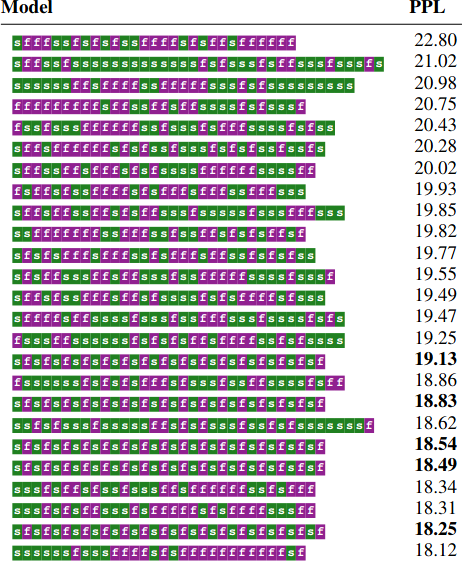
\includegraphics[scale=0.34]{img/sandwich_transformers_models2.png}
    \end{center}
\end{frame}




% MPNet
\section{MPNet}
\begin{frame}
    \frametitle{MPNet \cite{mpnet}}
    \begin{itemize}
        \item April 2020, Microsoft -- code available
        \item MPNet (masked and permuted language modeling) inherits the advantages of BERT (MLM) and XLNet (PLM) and avoids their limitations:
        \begin{itemize}
            \item BERT (MLM) - neglects dependency among predicted tokens
            \item XLNet (PLM) - does not leverage the full position information of a sentence (does not know the position information of the full sentence during the autoregressive pre-trainin)
        \end{itemize}
        \item MPNet outperforms MLM and PLM by a large margin, and achieves better results
    \end{itemize}
\end{frame}

\begin{frame}
    \frametitle{Unified view of MLM and PLM}
    \begin{center}
        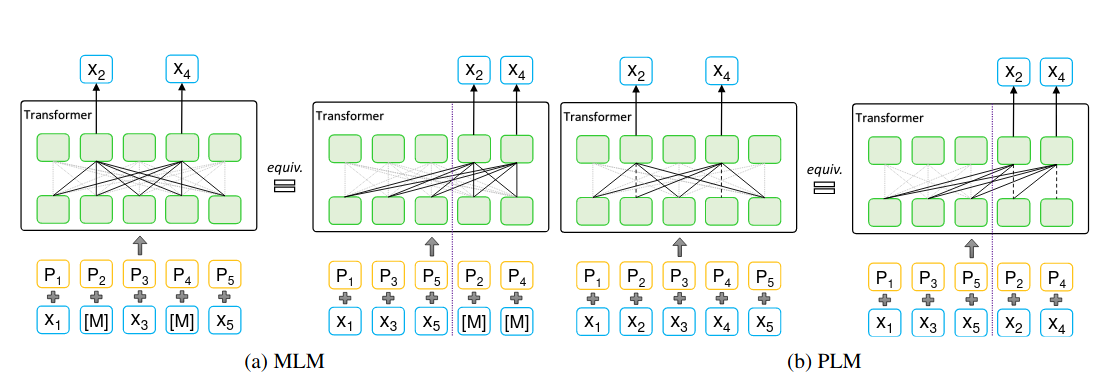
\includegraphics[scale=0.30]{img/mpnet_mlm_plm.png}
    \end{center}
\end{frame}

\begin{frame}
    \frametitle{Example}
    An example sentence \textbf{the task is sentence classification} to illustrate the conditional information of MLM, PLM and MPNet:
    \begin{center}
        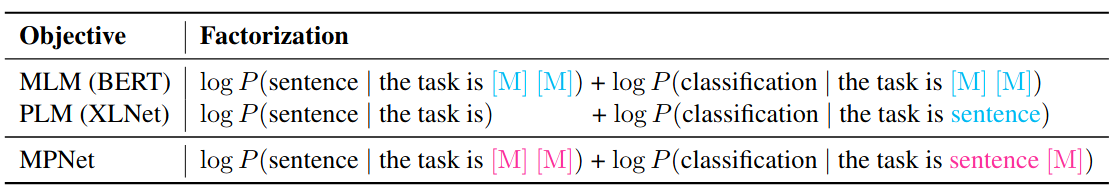
\includegraphics[scale=0.29]{img/mpnet_example.png}
    \end{center}
\end{frame}

\begin{frame}
    \frametitle{MPNet}
    \begin{center}
        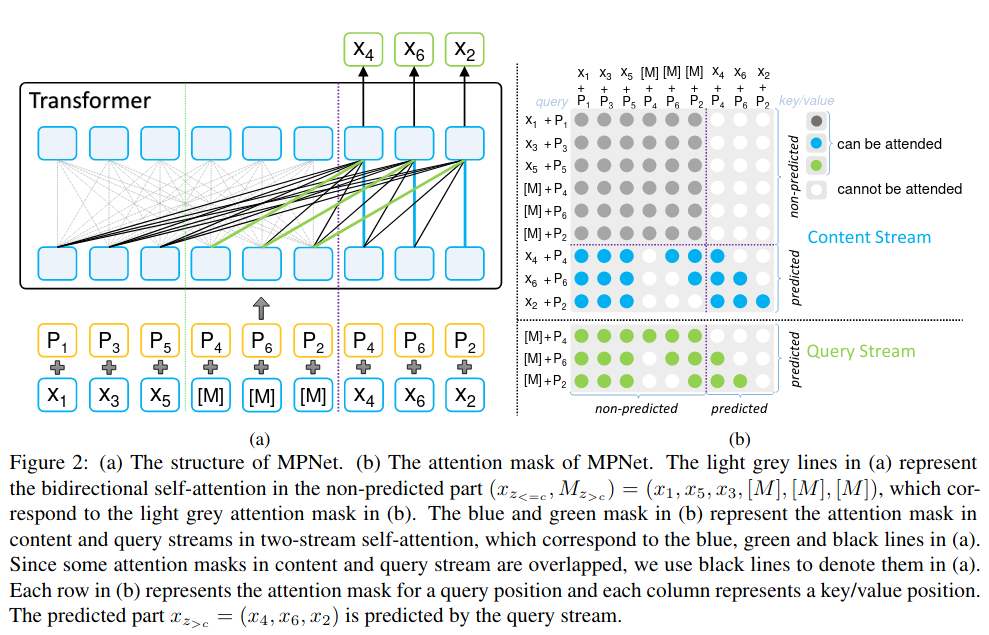
\includegraphics[scale=0.30]{img/mpnet.png}
    \end{center}
\end{frame}

\begin{frame}
    \frametitle{Score}
    \begin{center}
        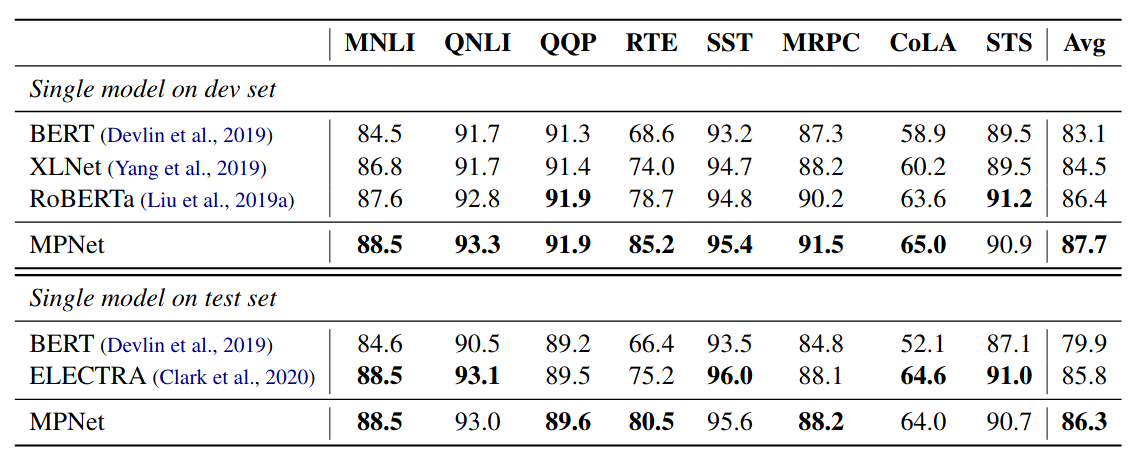
\includegraphics[scale=0.25]{img/mpnet_score.png}
    \end{center}
\end{frame}





% References
\section{References}
\begin{frame}[allowframebreaks,t]
    \tiny
    \frametitle{References}
    \bibliographystyle{ieeetr}
    \bibliography{sparse_transformers}
    %\nocite{*}
\end{frame}

\end{document}
